\documentclass[11pt]{scrartcl}

\usepackage[sexy]{evan}
\usepackage{import}
\usepackage[table]{xcolor}
\usepackage{xfp}

\newcommand{\gad}{\textcolor{yellow}{$\bigstar$}}
\newcommand{\bad}{\textcolor{red}{$\bigstar$}}

\definecolor{dcol0}{HTML}{C8E6C9}
\definecolor{dcol1}{HTML}{D4E9B3}
\definecolor{dcol2}{HTML}{E5ED9A}
\definecolor{dcol3}{HTML}{FFF59D}
\definecolor{dcol4}{HTML}{FFE082}
\definecolor{dcol5}{HTML}{FFCC80}
\definecolor{dcol6}{HTML}{FFAB91}
\definecolor{dcol7}{HTML}{F49890}
\definecolor{dcol8}{HTML}{E57373}
\definecolor{dcol9}{HTML}{D32F2F}

\makeatletter
\newcommand{\getcolorname}[1]{dcol#1}
\makeatother

\newcommand{\dif}[1]{%
    \edef\colorindex{\number\fpeval{floor(#1)}}%
    \edef\fulltext{#1}%
    \colorbox{\getcolorname{\colorindex}}{%
        \ifnum\colorindex>8
            \textbf{\textcolor{white}{\,\fulltext\,}}%
        \else
            \textbf{\textcolor{black}{\,\fulltext\,}}%
        \fi
    }%
}
% Variable para dificultad (inicial 0)
\newcommand{\thmdifficulty}{0}

% Comando para asignar dificultad antes del problema
\newcommand{\problemdiff}[1]{\renewcommand{\thmdifficulty}{#1}}

% Estilo del problema que incluye dificultad antes del título
\declaretheoremstyle[
    headfont=\color{blue!40!black}\normalfont\bfseries,
    headformat={%
      \dif{\thmdifficulty}\quad \NAME~\NUMBER\ifx\relax\EMPTY\relax\else\ \NOTE\fi
    },
    postheadspace=1em,
    spaceabove=8pt,
    spacebelow=8pt,
    bodyfont=\normalfont
]{problemstyle}

    \declaretheorem[style=problemstyle,name=Problema,sibling=theorem]{problema}
    \declaretheorem[style=problemstyle,name=Problema,numbered=no]{problema*}

\definecolor{yellow4}{RGB}{255, 206, 0}


\title {Angle Chasing}

\author{Emmanuel Buenrostro}


\begin{document}
\maketitle
\section{Herramientas}
El Angle Chasing (Cazar \'angulos) busca obtener la mayor informaci\'on posible de una configuraci\'on gracias a los \'angulos, una gran cantidad de problemas con esto obtienes la informaci\'on suficiente para terminarlos, y si no una gran parte de lo que ocupas. \\
Cazar los \'angulos muchas veces no es tan facil y puede ser lo unico necesario para resolver problemas muy complejos, todo si sabes como encontrarlos.
\\
Como tal no hay mucha teor\'ia como para un primer acercamiento a Angle Chasing, entonces quiero pensarlo m\'as como una caja de herramientas que puedes usar para encontrar/usar los \'angulos. 
\subsection{Triangulos, poligonos}

\begin{itemize}
\item    Los \'angulos interiores de un tri\'angulo suman $180^{\circ}$.


\item    Un \'angulo externo de un tri\'angulo es la suma de los dos \'angulos interiores opuestos.

\item    En general, la suma de los \'angulos internos de un poligono de $n$ lados es 
    $$180(n-2)$$

\item    En un tri\'angulo no degenerado $ABC$ se tiene que 
    $$AB=AC \Longleftrightarrow \angle ABC = \angle ACB$$

\end{itemize}

\subsection{Paralelas y opuestos por el vertice}
Estas son igualdades de \'angulos muy conocidas, no tengo mucho que agregar.
\begin{itemize}
    
   \item En esta imagen hay dos rectas paralelas y una recta que las intersecta, entonces los \'angulos rojos son iguales.
    \begin{center}
    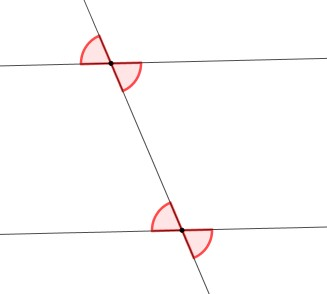
\includegraphics[scale=.5]{AC2.jpg}
    \end{center}
    A traves de un punto es opuestos por el vertice, a traves de las dos rectas paralelas es entre paralelas.
\end{itemize}

\subsection{Circulos}
Los circulos nos ayudan a mover muchos \'angulos, principalmente con lo siguiente.
\begin{theorem}
    [\'Angulos inscritos]
    Si el \'angulo $\angle ACB$ esta inscrito en el circulo (los 3 puntos estan en el circulo), entonces abre un arco de $2\angle ACB$.
    \begin{center}
        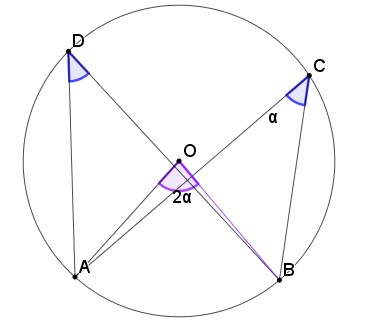
\includegraphics[scale=0.5]{AC3.jpg}
    \end{center}
\end{theorem}
Particularmente
\begin{theorem}
    Sea $M$ el punto medio del arco $AB$ que abre el \'angulo $\angle ACB$, entonces $CM$ es bisectriz de $\angle ACB$.
\end{theorem}
Esto sale aprovechando el isosceles que te da y moviendo los \'angulos con los arcos. \\
Ahora, estos \'angulos se suelen aprovechar mayormente con cierto tipo de cuadrilateros, los cuadrilateros ciclicos.
\begin{definition}
    Se dice que un cuadrilatero $ABCD$ es ciclico si y solo si $A,B,C,D$ estan en una misma circunferencia.
\end{definition}


Y entonces las siguientes tres condiciones son equivalentes en un cuadrilatero $ABCD$ (es decir, si una se cumple se cumplen todas y si una no se cumple ninguna se cumple). 
\begin{itemize}
    \item $ABCD$ es ciclico
    \item $\angle ABC+\angle CDA=180$
    \item $\angle ABD=\angle ACD$
\end{itemize}
En particular quiero enfatizar el uso de los \'angulos inscritos en los cuadrilateros ciclicos, ya que tienes muchos \'angulos que abren los mismos arcos y por lo tanto son iguales (En esto se usa el 3er punto).
\begin{example}
    Sea $ABCD$ un cuadrilatero ciclico. Sea F el punto medio del arco $AB$ que no contiene a $C$ ni a $D$. Las lineas $DF$ y $AC$ se intersecan en $P$ y las lineas $CF$ y $BD$ se intersecan en $Q$. Demuestra que $PQ$ y $AB$ son paralelas.
\end{example}
\begin{soln}
    \begin{center}
        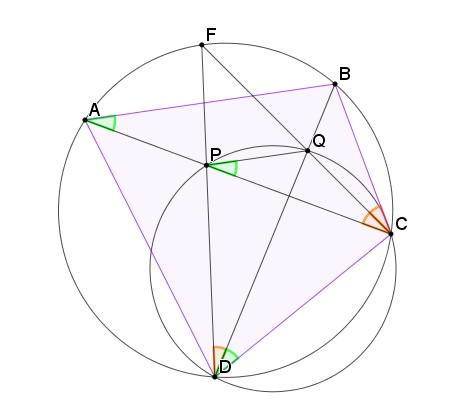
\includegraphics[scale=0.8]{Img5.jpg}
    \end{center}
    Como $F$ es el punto medio del arco $AB$ entonces $\angle BCF=\angle FCA$ y por lo tanto
    $$\angle QDP=\angle BDF=\angle BCF=\angle FCA=\angle QCP$$
    Por lo que $QPCD$ es ciclico y entonces 
    $$\angle CPQ=\angle CDQ=\angle CDB=\angle CAB$$
    Por lo que son paralelas.
\end{soln}
\begin{theorem}
     Si tienes un triangulo $ABC$ inscrito en un circulo $\omega$ con centro $O$ y un punto $P$ entonces estos 3 son equivalentes:
\begin{itemize}
    \item $PA$ es tangente a $\omega$
    \item $OA \perp PA$
    \item $\angle PAB=\angle ACB$
\end{itemize}
\end{theorem}


\subsection{H y 0}
    Si trazamos las alturas $AD,BE,CF$ y el ortocentro $H$ nos quedan los siguientes \'angulos (Mismo color es que son iguales).
    \begin{center}
        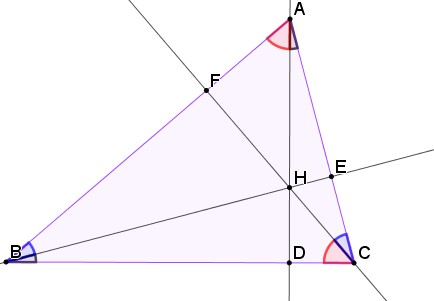
\includegraphics[scale=0.8]{AC6.jpg}
    \end{center}
    Esto por los distintos ciclicos que se forman por los \'angulos de 90 (Adem\'as dos angulos de 90 suman 180). \\
    Estos ciclicos son: 
    $$AEHF, CDHE, BFHD, AEDB, CDFA, BFEC$$
    Adem\'as estos nos dan que $H$ es el incentro de $DEF$. 
    \begin{definition}
        En un triangulo dos rectas se llaman isogonales si pasan por un vertice y son reflejadas respecto a la bisectriz de ese vertice. 
    \end{definition}
    \begin{theorem}
        En un triangulo $ABC$, se cumple que $AH, AO$ son isogonales.
    \end{theorem}
    \begin{proof}
        Se tiene que $\angle BAH=90-\angle B$ y adem\'as $\angle AOC=2\angle B$ y como $OA=OC$ entonces $\angle CAO=\frac{180-2\angle B}{2}=90-\angle B$, entonces como el \'angulo es el mismo son isogonales.
    \end{proof}

 
\subsection{Reflejar}
    Podemos reflejar principalmente sobre un punto o sobre una recta. \\
    Reflejar sobre un punto $P$ es agarrar todos los punto $X$ del plano y mandarlos al punto $X'$ tal que $P$ es el punto medio de $XX'$ (en otras palabras, tomas la distancia de $XP$ y usas la misma distancia pero en el lado contrario). \\
    Reflejar sobre una recta $l$ es agarrar todos los puntos $X$ del plano y mandarlos al punto $X'$ tales que $l$ es la mediatriz de $XX'$ (en otras palabras tomar la distancia a la recta y usarla pero en el lado contrario) \\
    Reflejar cumple que si reflejas dos veces es como si no hubieras hecho nada. \\
    Hacer reflexiones puede ser muy util en Angle Chasing para dos cosas, poder igualar \'angulos sabiendo que cierta parte del dibujo es el reflejo de otra parte del dibujo, o para crear puntos/trazos auxiliares con ciertas propiedades y que te pueden dar ciclicos, paralelas, u otro tipo de informaci\'on.  \\
    \begin{theorem}
    En un triangulo $ABC$ con ortocentro $H$, punto medio de $BC$ $M$, $X$ la reflexi\'on de $H$ sobre $BC$, $Y$ la reflexi\'on de $H$ sobre $M$. Se cumple que 
    $AY$ es diametro de el circuncirculo y que $X$ esta en el circuncirculo.
    \end{theorem}
    \begin{proof}
        .
        \begin{center}
         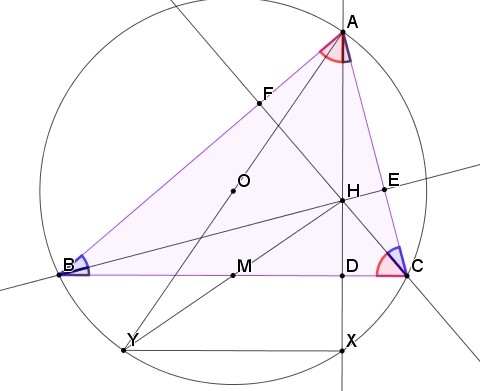
\includegraphics[scale=0.5]{AC7.jpg}
        \end{center}
        Se puede calcular que $\angle BHC=180-\angle A$ entonces $\angle BXC=180-\angle A$, asi que $BXCA$ es ciclico. \\
        Y como $MH=MY$ y $MB=MC$ entonces $HBYC$ es un paralelogramo y $\angle BYC=180-\angle A$ asi que $BYCA$ tambien es ciclico. \\
        Y como $MD || YX$ por tales, entonces $\angle YXA=\angle MDH=90$, entonces $AY$ es diametro.
    \end{proof}
    Como se acaba de mostrar una reflexi\'on muy util es reflejar sobre algun punto medio para obtener paralelogramos, otro ejemplo es:
    \begin{example}
        
    Sea $ABC$ un triángulo acutángulo con $AB \neq AC$, $M$ el punto medio de $BC$ y $H$ el
ortocentro de $ABC$. La circunferencia que pasa por $B$, $H$ y $C$ corta a la mediana $AM$ en
$N$. Muestra que $\angle ANH = 90^o$.
    
    \end{example}
    \begin{soln}
    \begin{center}
        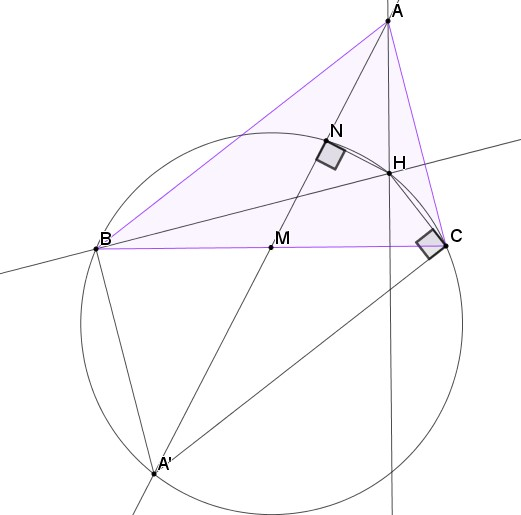
\includegraphics[scale=0.5]{AC5.jpg}
    \end{center}
        Sea $A'$ la reflexi\'on de $A$ sobre $M$, en particular $BACA'$ es un paralelogramo porque $MB=MC$ y $MA=MA'$. Entonces $\angle BA'C=\angle A$ y 
        $$\angle BHC =180-\angle HBC-\angle HCB=180-90+\angle C-90+\angle B=180-\angle A$$
        Por lo que $BHCA'$ es ciclico. Y como $\angle (HC, CA')=(HC,AB)=90$ por las paralelas, entonces el ciclico $NHCA'$ tiene diametro $A'H$ y $\angle A'NH=90$ y $\angle ANH=90$
    \end{soln}

    Otra reflexi\'on muy util en triangulos es reflejar sobre alguna bisectriz. 
    \begin{example}
        Sea $ABC$ un triangulo con circuncentro $O$ y ortocentro $H$. Prueba que $AO=AH$ si y solo si $\angle BAC=60$
    \end{example}
    \begin{soln}
    .
        \begin{center}
            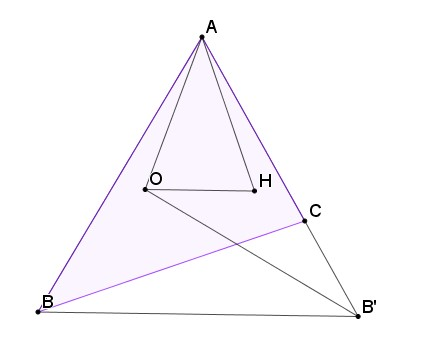
\includegraphics[scale=0.5]{Img16.jpg}
        \end{center}
        Si $AO=AH$ sucede que: \\
        Como $\angle BAO=\angle CAH$, entonces al reflejar $O$ sobre la bisectriz de $\angle BAC$ nos queda $H$, y digamos que al reflejar $B$ nos queda $B'$. Entonces 
        $$\angle (B'O, AB)=\angle (BH, AB')=90$$
        Asi que $B'$ esta en la mediatriz de $AB$ y entonces $AB=AB'=BB'$ generando un triangulo equilatero y el \'angulo de 60 necesario. 
        (El regreso es practicamente analogo.)
    \end{soln}

\subsection{Incentro-Excentro}



\newpage
\section{Problemas}
\epigraph{" i'm not ready at all but it's now august 2 and THE SHOW MUST GO ON"
}{Evan Chen}

\problemdiff{3}
\begin{problem}
    Sea $ABC$ un triangulo. El incirculo de $ABC$ es tangente a $AB, AC$ en $D,E$. Sea $O$ el circuncentro de $BCI$. Demuestra que $\angle ODB=\angle OEC$
\end{problem}

\problemdiff{1}
\begin{problem}
    Sea $t$ una tangente por el vertice $C$ al circuncirculo de un triangulo $ABC$. Una recta $p$ paralela a $t$ intersecta $BC,AC$ en los puntos $D,E$. Demuestra que $A,B,D,E$ son conciclicos. 
\end{problem}



\problemdiff{2}
\begin{problem} 
    Sea $ABCD$ un cuadrado y sea $Y$ un punto dentro de la diagonal $AC$ distinto del punto medio de $AC$. La recta perpendicular al segmento $BY$ que pasa por $Y$ corta a la recta $AD$ en $X$ y a la recta $CD$ en $Z$. Muestra que $AX=CZ$. 
\end{problem}

\problemdiff{2}
\begin{problem} [Recta de Simson] 
    Sea $ABC$ un triangulo y sea $P$ cualquier punto en su circuncirculo. Sea $X,Y,Z$ los pies de altura desde $P$ hasta $BC,CA$ y $AB$. Prueba que los puntos $X,Y,Z$ son colineales.
\end{problem}

\problemdiff{2}
\begin{problem}
    Sea $I$ el incentro de un triangulo $ABC$ con $AB<AC$. La linea $AI$ intersecta el circuncirculo de $ABC$ en $D$. El circuncirculo de $CDI$ intersecta $BI$ de nuevo en $K$. Prueba que $BK=CK$.
\end{problem}



\problemdiff{2.5}
\begin{problem}
    En un triangulo rectangulo $ABC$ con $\angle A=90, \angle C=30$. Sea $\omega$ el circulo que pasa por $A$ y es tangente a $BC$ en el punto medio. $\omega$ intersecta $AC$ en $N$ y al circuncirculo de $ABC$ en $M$. Prueba que $MN \perp BC$.
\end{problem}

\problemdiff{3}
\begin{problem} %OMM 2011/2    
    Sea $ABC$ un triángulo acutángulo con vértices sobre una circunferencia $\Gamma$. Sea $\ell$ la recta
tangente a $\Gamma$ en $A$. Sean $D$ y $E$ los puntos de intersección de la recta $\ell$ y del segmento $AC$ con la circunferencia de centro $B$ y radio $BA$, respectivamente. Muestra que $DE$ pasa por el ortocentro del triángulo $ABC$.
    
\end{problem}

\problemdiff{3}
\begin{problem}%OMM 2021/4}
    Sea $ABC$ un triángulo acutángulo escálelo con $\angle BAC=60^{\circ}$ y ortocentro $H$. Sean $\omega_b$ la circunferencia que pasa por $H$ y es tangente a $AB$ en $B$, y $\omega_c$ la circunferencia que pasa por $H$ y es tangente a $AC$ en $C$. Prueba que $\omega_b$ y $\omega_c$ solamente tienen a $H$ como punto común.  Prueba que la recta que pasa por $H$ y el circuncentro $O$ del triángulo $ABC$ es una tangente común a $\omega_b$ y $\omega_c$.
 
\end{problem}

\problemdiff{4}
\begin{problem} %USAMO 2023/1
    En un triangulo acutangulo $ABC$, sea $M$ el punto medio de $BC$. Sea $P$ el pie de altura de $C$ hacia $AM$. Supon que el circuncirculo de el triangulo $ABP$ intersecta la linea $BC$ en $B$ y $Q$.Sea $N$ el punto medio de $AQ$. Muestra que $NB=NC$.
\end{problem}



\problemdiff{5}
\begin{problem} [\gad] %USA TSTST 2023/1 creo
    Sea $ABC$ un triangulo con gravicentro $G$. Los puntos $R$ y $S$ estan en los rayos $GB$ y $GC$, tal que 
    $$\angle ABS=\angle ACR=180-\angle BGC$$
    Prueba que $\angle RAS+\angle BAC=\angle BGC$
\end{problem}

\problemdiff{5}
\begin{problem}
    Sea $ABC$ un triangulo acutangulo, sea $D$ el pie de altura desde $C$. La bisectriz de $\angle ABC$ intersecta $CD$ en $E$ e intersecta al circuncirculo $\omega$ de $ADE$ en $F$. Si $\angle ADF=45$ muestra que $CF$ es tangente a $\omega$.
\end{problem}


\problemdiff{6}
\begin{problem}
  Sea $ABCD$ un cuadrilatero inscrito en el circulo $\omega$ con $AC \perp BD$. Sean $E,F$ las reflexiones de $D$ sobre $BA$ y $BC$, respectivamente, sea $P$ la intersecci\'on de las lineas $BD$ y $EF$. El circuncirculo de $EPD$ intersecta $\omega$ en $D$ y $Q$ y el circuncirculo de $FPD$ intersecta $\omega$ en $D$ y $R$. Demuestra que $EQ=FR$.
\end{problem}


\end{document}